\documentclass[border=10pt]{standalone}
\usepackage{tikz}
\usetikzlibrary{arrows.meta,positioning,calc}

\begin{document}
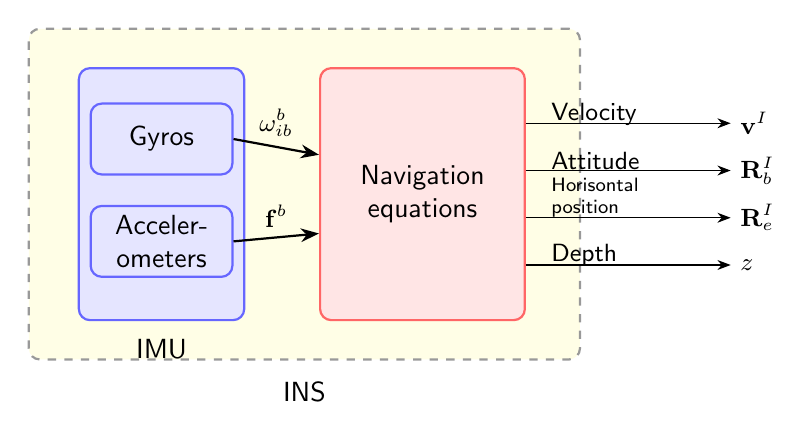
\begin{tikzpicture}[
    font=\sffamily,
    >=Stealth,
    block/.style={draw,rounded corners,thick,align=center},
    imuBlock/.style={block,fill=blue!10,draw=blue!60},
    navBlock/.style={block,fill=red!10,draw=red!60},
    insBlock/.style={block,fill=yellow!10,draw=black!40,
                     dashed,rounded corners=4pt,thick},
    smalltext/.style={font=\scriptsize\sffamily},
    labeltext/.style={font=\small\sffamily},
    mathlabel/.style={font=\small}
]

% Overall INS dashed box
\node[insBlock,minimum width=7cm,minimum height=4.2cm,anchor=west] (INS) at (0,0) {};
\node[below=0.15cm of INS.south] {\sffamily INS};

% IMU block inside INS (left)
\node[imuBlock,minimum width=2.1cm,minimum height=3.2cm] (IMU) at ([xshift=1.7cm]INS.west) {};
\node[below=0.1cm of IMU.south] {\sffamily IMU};

% Gyros and Accelerometers blocks inside IMU
\node[imuBlock,minimum width=1.8cm,minimum height=0.9cm] (gyros) at ([yshift=0.7cm]IMU.center) {\sffamily Gyros};

\node[imuBlock,minimum width=1.8cm,minimum height=0.9cm] (accel) at ([yshift=-0.6cm]IMU.center)
        {\sffamily Acceler-\\ometers};

% Navigation equations block
\node[navBlock,minimum width=2.6cm,minimum height=3.2cm,
      right=2.0cm of IMU.center] (NAV) {\sffamily Navigation\\equations};

% Arrows from IMU to NAV
\draw[->,thick] (gyros.east) -- node[above,mathlabel] {$\boldsymbol{\omega}^b_{ib}$}
      ($(NAV.west)+(0,0.5)$);

\draw[->,thick] (accel.east) -- node[above,mathlabel] {$\mathbf{f}^b$}
      ($(NAV.west)+(0,-0.5)$);

% Right-hand output arrows from NAV
% Define output y positions relative to NAV
\coordinate (vpos)  at ($(NAV.east)+(0,0.9)$);
\coordinate (apos)  at ($(NAV.east)+(0,0.3)$);
\coordinate (hpos)  at ($(NAV.east)+(0,-0.3)$);
\coordinate (dpos)  at ($(NAV.east)+(0,-0.9)$);

% Velocity
\draw[->] (vpos) -- ++(2.6,0) node[right,mathlabel] {$\mathbf{v}^I$};
\node[labeltext,anchor=west] at ($(vpos)+(0.2,0.12)$) {Velocity};

% Attitude
\draw[->] (apos) -- ++(2.6,0) node[right,mathlabel] {$\mathbf{R}^I_b$};
\node[labeltext,anchor=west] at ($(apos)+(0.2,0.12)$) {Attitude};

% Horizontal position (two-line label, note original misspelling)
\draw[->] (hpos) -- ++(2.6,0) node[right,mathlabel] {$\mathbf{R}^I_e$};
\node[smalltext,anchor=west,align=left] at ($(hpos)+(0.2,0.25)$)
      {Horisontal\\position};

% Depth
\draw[->] (dpos) -- ++(2.6,0) node[right,mathlabel] {$z$};
\node[labeltext,anchor=west] at ($(dpos)+(0.2,0.12)$) {Depth};

\end{tikzpicture}
\end{document}